\section{Second phase with regular bins}

Let $\calE$ resp. $\calR$ be the set of empty resp. regular bins at
the beginning of the second phase, and let $e=|\calE|$. Let
$\lambda\in\{0,1,2,3\}$ be such that $|\calR|=3e+\lambda$;
Lemma~\ref{l:1}(\ref{i1:er}) implies that $\lambda$ exists. Note
that it is possible that $\calR=\emptyset$, in that case $e=\lambda=0$.

We organize the remaining non-complete bins into blocks $\calB_i$, and
then order them into a list $\calL$, as follows:

\begin{dfn}\label{d:blocks}
Denote the empty bins $E_1, E_2, \dots, E_e$.  The regular
bins are denoted by $R_{i,j}$, $i=1,...,e+1$, $j=1,2,3$. The $i$th
\textbf{block} $\calB_i$ consists of bins $R_{i,1},R_{i,2},R_{i,3},E_i$ in this
order. There are several modifications to this rule:
\begin{compactenum}[\rm (1)] 
\item The first block $\calB_1$ contains
only $\lambda$ regular bins, i.e., it contains $R_{1,1},\ldots,R_{1,\lambda},E_1$ in this
order; in particular, if $\lambda=0$ then $\calB_1$ contains only
$E_1$.

\item The last block $\calB_{e+1}$ has no empty bin,
only exactly $3$ regular bins. 

\item If $e=0$ and $r=\lambda>0$ we define only a single block $\calB_1$
which contains $r=\lambda$ regular bins $R_{1,1},\ldots,R_{1,\lambda}$. 

\item If $e=r=\lambda=0$, there is no block, as there are no empty and
  regular bins. 

\item  If $r>0$, we choose as the first regular bin the one with
size at most $4$, if there is such a bin. 
\end{compactenum}
Denote the first regular bin by $\Rbar$.  If no regular bin exists
(i.e., if $r=0$), $\Rbar$ is undefined.
\end{dfn}
Note that $\Rbar$ is either the first bin $R_{1,1}$ in $\calB_1$ if
$\lambda>0$ or the first bin $R_{2,1}$ in $\calB_2$ if $\lambda=0$. By
Lemma~\ref{l:1}(\ref{i1:tiny}) there exists at most one regular bin
with size at most $4$, thus all the remaining $R_{i,j}\neq\Rbar$ have
$s(R_{i,j})>4$.
\begin{dfn}\label{d:list}
The \textbf{list of bins} $\calL$ we use in the second phase contains first the
special bins and then all the blocks $\calB_1$, \ldots, $\calB_{e+1}$.
Thus the list $\calL$ is (some or all of the first six bins may not
exist):
\[
L, M, T, R_{1,1}, R_{1,2}, R_{1,3}, E_1, R_{2,1}, R_{2,2}, R_{2,3},
E_2, \dots,
E_e,  R_{e+1,1}, R_{e+1,2}, R_{e+1,3}.
\]
\end{dfn}
Whenever we refer to the ordering of the bins, we mean the ordering in
the list $\calL$. See Figure~\ref{fig:1} for an illustration.

\begin{figure}[th]
\begin{center}
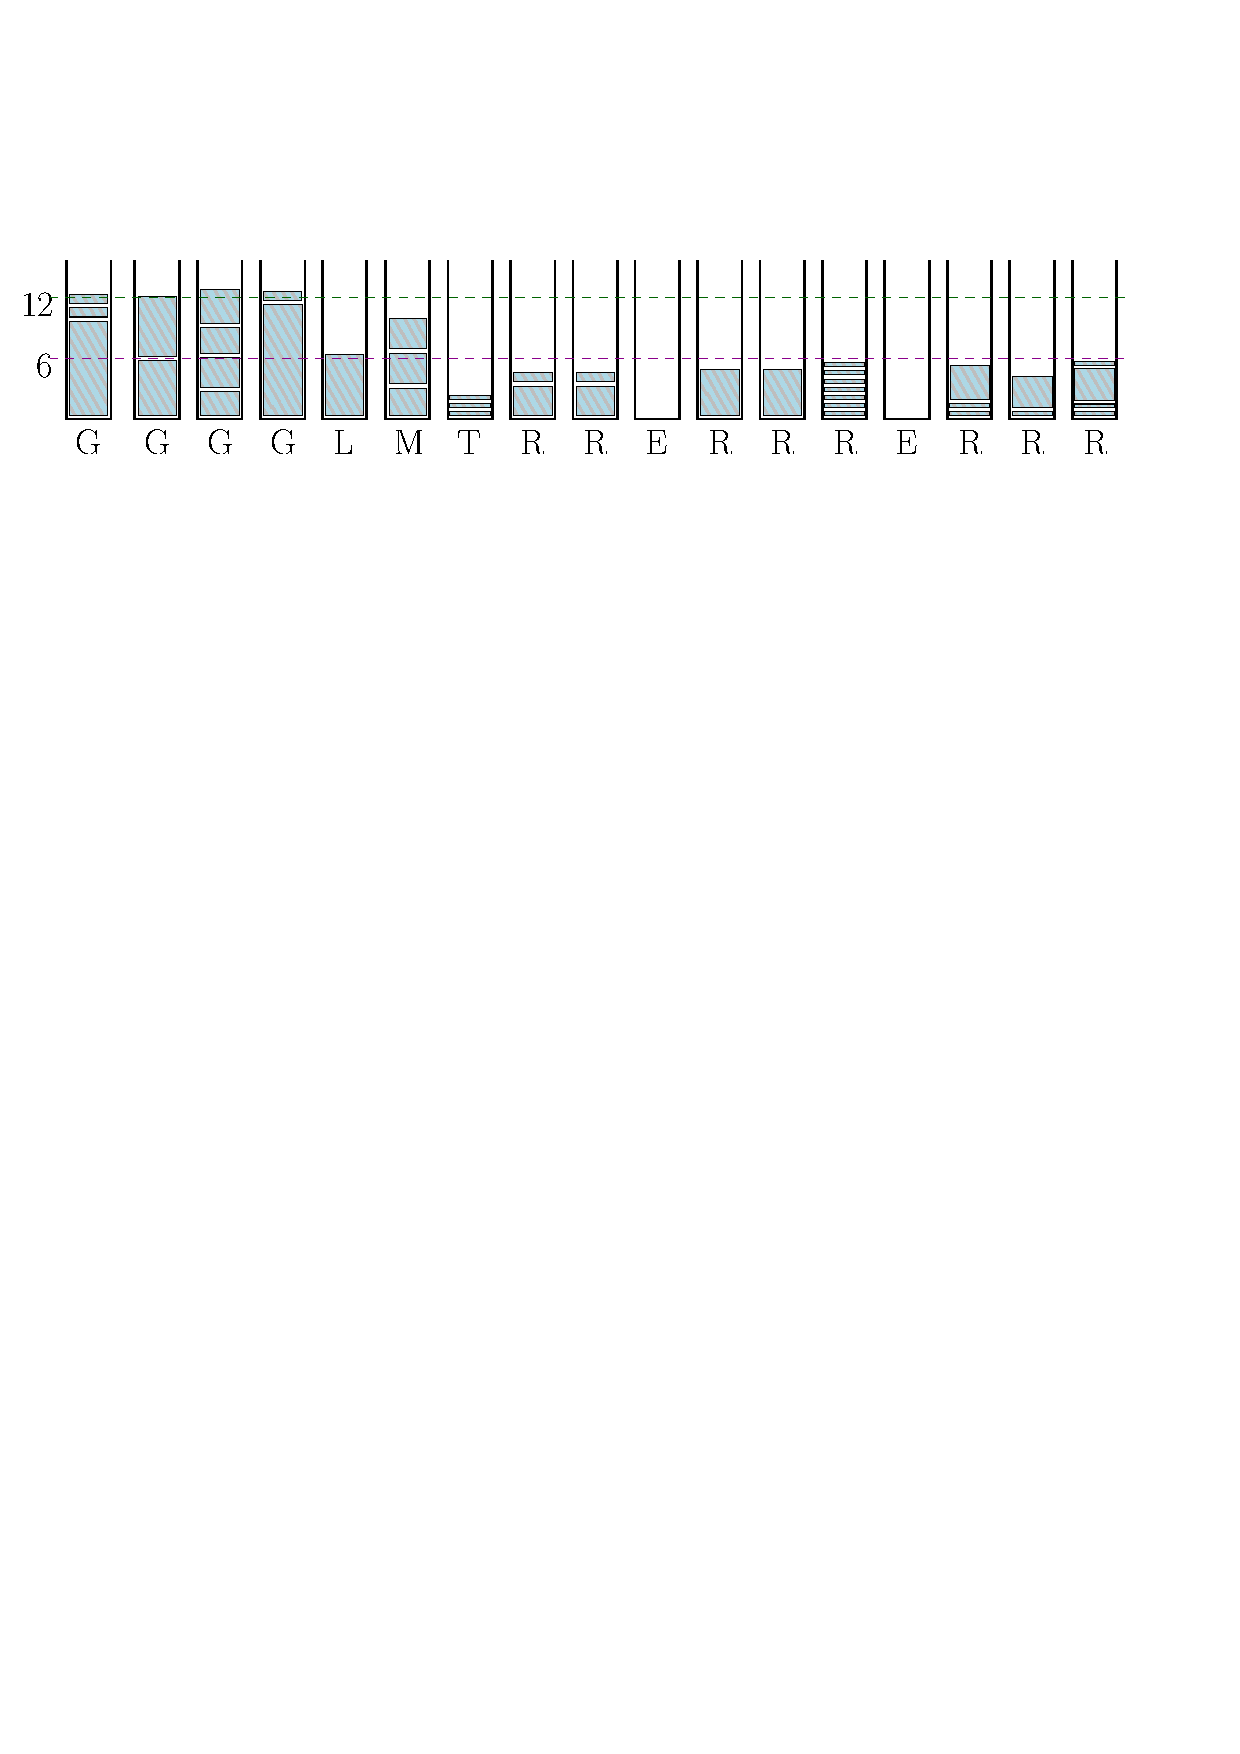
\includegraphics[width=\textwidth]{img/first_phase.pdf}
\end{center}
\caption{A typical state of the algorithm after the first phase. The bin labels correspond to the particular bin types. $G$ denotes complete bins, other labels are the initial letters of the bin types. The non-complete bins (other than $G$) are ordered as in
  the list $\calL$ at the beginning of the second phase with regular
  bins.}
\label{fig:1}
\end{figure}

\algobox{{\bf Algorithm for the second phase with regular bins:}

Let $\calL$ be the list of bins as in Definition~\ref{d:list}, with
all bins of capacity 18. 

\begin{compactenum}[(1)]

\item For any incoming item $i$:
\item \indentskip If $i$ is huge, pack it using First Fit on the
  reverse of the list $\calL$.
\item \indentskip In all other cases, pack $i$ using First Fit on the normal list $\calL$.
\end{compactenum}
}

Suppose that we have an instance that has a packing into bins of
capacity 12 and on which our algorithm fails. We may assume that the
algorithm fails on the last item. Let us denote this item by $f$.
We have $s(f)>6$, as otherwise all bins have size more than 12,
contradicting the existence of optimal packing.
Call the items that arrived in the second phase {\em new} (including
$f$), the items from the first phase are {\em old}.
See Figure~\ref{fig:2} for an illustration of a typical final
situation (and also of notions that we introduce later).

Our overall strategy is to obtain a contradiction by showing that  
$$w(\calL)+w(f)>0\,.$$ 
In some cases, we instead argue that
$v(\calL)+v(f)>0$ or $s(\calL)+s(f)>12|\calL|$. Any of these is
sufficient for a contradiction, as all complete bins have both
value and weight nonnegative and size at least 12.

Let $\calH$ denote all the bins from $\calL$ with a huge item,
and let $\hmodfour=|\calH| \bmod 4$. First
we show that the average size of bins in $\calH$ is large and exclude
some degenerate cases; in particular, we exclude the case when no
regular bin exists.

\begin{lem}
\label{l:huge} 
Let $\rho$ be the total size of old items
in $\Rbar$ if $\calR\neq\emptyset$ and $\Rbar\in\calH$, otherwise set $\rho=4$.
\begin{compactenum}[\rm (i)]
\item \label{i:hspecial} 
The bins $\calH$ are a final segment of the list $\calL$ and
$\calH\subsetneq\calE\cup\calR$. In particular, $\calR\neq\emptyset$
and $\Rbar$ is defined.
\item \label{i:hr}
We have
$s(\calH)\geq12|\calH|+\hmodfour+\rho-4$. 
\item \label{i:h}
If $\calH$ does not include $\Rbar$, then
$s(\calH)\geq12|\calH|+\hmodfour\geq12|\calH|$. 
\item \label{i:hfirst}
If $\calH$ includes $\Rbar$, then
$s(\calH)\geq12|\calH|+\hmodfour-1\geq12|\calH|-1$.
\end{compactenum} 
\end{lem}
\begin{proof}
First we make an easy observation used later in the proof. If
$\calE\cup\calR\cup\{T\}$ contains a bin $B$ with no huge item,
then no bin preceding $B$ contains a huge item.  Indeed, if a huge
item does not fit into $B$, then $B$ must contain a new item $i$ of
size at most $9$. This item $i$ was packed using First Fit on the
normal list $\calL$, and therefore it did not fit into any previous
bin. Thus the huge item also does not fit into any previous bin, and
cannot be packed there.

Let $\calH'=\calH\cap(\calE\cup\calR)$. We begin proving our lemma for
$\calH'$ in place of $\calH$.  That is, we ignore the special bins at
this stage. 
The previous observation shows that $\calH'$ is a final segment of the
list.

We now prove the claims (\ref{i:hr})--(\ref{i:hfirst}) with
$\calH'$ in place of $\calH$. 
All bins $R_{i,j}$ with a huge item have size at least $4+9=13$, with
a possible exception of $\Rbar$ which has size at least
$\rho+9=13+\rho-4$, by the definition of $\rho$. Each $E_i$ with a
huge item has size at least $9$. Thus for each $i$ with
$E_i\in\calH'$, $s(E_i)+s(R_{i+1,1})+s(R_{i+1,2})+s(R_{i+1,3})\geq
4\cdot 12$, with a possible exception of $i=1$ in the case when
$\lambda=0$. Summing over all $i$ with $E_i\in\calH'$ and the $\hmodfour$
bins in $\calR$ from the first block intersecting $\calH'$, and
adjusting for $\Rbar$ if $\Rbar\in\calH'$, (\ref{i:hr}) for $\calH'$
follows. The claims (\ref{i:h}) and (\ref{i:hfirst}) for $\calH'$ are
an immediate consequence as $\rho>3$ if $\Rbar\in\calH'$ and $\rho=4$
otherwise.

We claim that the lemma for $\calH$ follows if
$\calH'\subsetneq\calE\cup\calR$. Indeed, following the observation at
the beginning of the proof, the existence of a bin in $\calE\cup\calR$
with no huge item implies that no special bin has a huge item, i.e.,
$\calH'=\calH$, and also $\calH'=\calH$ is a final segment of
$\calL$. Furthermore, the existence of a bin in $\calE\cup\calR$
together with $3e\leq r$ implies that there exist at least one regular
bin, thus also $\Rbar$ is defined and (\ref{i:hspecial}) follows.
Claims (\ref{i:hr}), (\ref{i:h}), and (\ref{i:hfirst}) follow from
$\calH'=\calH$ and the fact that we have proved them for $\calH'$.

Thus it remains to show that $\calH'\subsetneq\calE\cup\calR$.
Suppose for a contradiction that $\calH'=\calE\cup\calR$.

If $T$ exists, let $o$ be the total size of old items in $T$. If also
$\Rbar$ exists, Lemma~\ref{l:1}(\ref{i1:tiny}) implies that
$o+\rho>6>4$, otherwise $o+\rho>4$ trivially. In either case, summing
with (\ref{i:hr}) we obtain
\begin{equation}\label{eq:Told}
  o+s(\calH')>12|\calH'|\,.
\end{equation}

Now we proceed to bound $s(\calH)$. We have already shown claim
(\ref{i:hfirst}) for $\calH'$, i.e., $s(\calH')\geq12|\calH'|-1$. If $L$ or
$M$ has a huge item, the size of the bin is at least 12, as there is
an old large or medium item in it. If $T$ has a huge item, then
(\ref{eq:Told}) implies $s(T)+s(\calH')>9+
o+s(\calH')>9+12|\calH'|$. Summing these bounds we obtain

\begin{equation}
s(\calH) > 12|\calH|-3 \,. \label{eq:T}
\end{equation}
 
We now derive a contradiction in each of the following four cases.

\mycase{Case 1:} All special bins have a huge item.  Then
$\calL=\calH$ and (\ref{eq:T}) together with $s(f)>6$ implies
$s(\calL)+s(f)>12|\calL|+3$, a contradiction.

\mycase{Case 2:} There is one special bin with no huge item.  Then its
size together with $f$ is more than 18, thus (\ref{eq:T}) together
with $s(f)>6$ implies $s(f)+s(\calL)>18+12|\calH|-3>12|\calL|$, a
contradiction.

\mycase{Case 3:} There are two special bins with no huge item and these
bins are $L$ and $M$.

Suppose first that $M$ contains a new item $n$. Then $s(L)+s(n)>18$ by
the First Fit packing rule. The bin $M$ contains at least one old
medium item.  Thus, using (\ref{eq:T}), we get
$s(f)+s(\calL)>6+s(L)+s(n)+3+12|\calH|-3> 24+ 12|\calH|=12|\calL|$, a
contradiction.

If $M$ has no new item, then either $f$ is huge and $M$ has at least
two medium items, or $f$ is large and $M$ has at least three items. In
both cases $v(M)+v(f)\geq 2$. Also $v(L)\geq -1$ since $L$ has a large
item, and $v(\calH)\geq0$ as each bin has a huge item. Altogether we
get that the total value $v(\calL)>0$, a contradiction.

\mycase{Case 4:} There are two or three special bins with no huge
item, one of them is $T$. Observe that the bin $T$ always contains a
new item $n$, as the total size of all old items in it is at most $3$. 

If there are two special bins with no huge item, denote the first one by
$B$. As we observed at the beginning of the proof, if $T$ exists and
has no huge item, no special bin can contain a huge item, thus the
third special bin cannot exist. We have
$s(B)+s(n)>18$, summing with (\ref{eq:Told}) we obtain
$s(f)+s(\calL)\geq
s(f)+s(B)+s(n)+o+s(\calH')>6+18+12|\calH'|=12|\calL|$, a contradiction.

If there are three special bins with no huge item, we have
$s(f)+s(L)>18$ and $s(M)+s(n)>18$. Summing with (\ref{eq:Told}) we
obtain $s(f)+s(\calL)>18+18+o+s(\calH')>36+12|\calH'|=12|\calL|$, a
contradiction.
%\qed
\end{proof}

Having proven Lemma~\ref{l:huge}, we can infer existence of the following
two important bins, which (as we will later see) split the instance into three
logical blocks:

\begin{dfn} ~ 

\begin{compactitem} \label{d:fc}
\item Let $F$, the \textbf{final bin} be the last bin in $\calL$ before
$\calH$, or the last bin if $\calH=\emptyset$.
\item Let $C$, the \textbf{critical bin}, be the
first bin in $\calL$ of size at most 12. 
\end{compactitem}
\end{dfn}

First note that both $F$ and $C$ must exist: $F$ exists by
Lemma~\ref{l:huge}(\ref{i:hspecial}), which also shows that
$F\in\calE\cup\calR$. $C$ exists, as otherwise the total size is more
than $12m$.

To make our calculations easier, we modify the packing so that $f$ is put
into $F$, even though it exceeds the capacity of $F$.
Thus $s(F)>18$ and $f$ (a new item) as well as all the other new items packed
in $F$ or in some bin before $F$ satisfy the property that they do not
fit into any previous bin.  See Figure~\ref{fig:2} for an illustration
of the definitions.

We start by some easy observations. Each bin, possibly with the
exception of $L$ and $M$, contains a new item, as it enters the phase
with size at most 6, and the algorithm failed. Only items of size at
most $9$ are packed in bins before $F$; in $F$ itself only the item
$f$ can be huge.  The bin $F$ always has at least two new items, one that did
fit into it and $f$. All the new items in the bins after $C$ are
large, except for the new huge items in $\calH$ and $f$ which can be
large or huge. (Note that at this point of the proof it is possible
that $C$ is after $F$; we will exclude this possibility soon.)

\begin{figure}[th]
\begin{center}
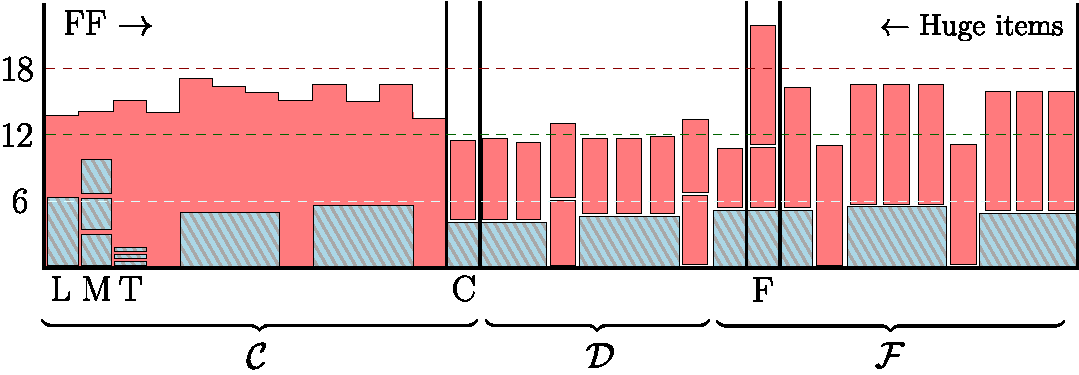
\includegraphics[width=1\textwidth]{img/second_phase.pdf}
\end{center}
\caption{A typical state of the algorithm after the second phase with regular
  bins. The gray (hatched) areas denote the old items (i.e., packed in
  the first phase), the red (solid) regions and rectangles denote the
  new items (i.e., packed in the second phase). The bins that are
  complete at the end of the first phase are not shown. The item $f$
  on which the algorithm fails is shown as packed into the final bin
  $F$ and exceeding the capacity $18$, following the convention
  introduced after Definition~\ref{d:fc}.}
\label{fig:2}
\end{figure}

More observations are given in the next two lemmata.

\begin{lem}
\label{l:aux}
\begin{compactenum}[(i)]
\item
\label{i:9}
Let $B$ be any bin before $F$. Then $s(B)>9$. Furthermore, if
$B\in\calE$ then $B$ contains at least two new items.
\item
\label{i:12}
Let $B,B',B''$ be any three bins in the ordering $\calL$ with
$B <_{\calL} B' <_{\calL} B'' \leq_{\calL} F$ and let $B''$ contain at least two new items. Then
$s(B)+s(B')+s(B'')>36+o$, where $o$ is the size of old items in $B''$.
\item  
\label{i:11}
Let $B$ be arbitrary and let $B'\in\calR$ be a bin such that $B <_{\calL} B' \leq_{\calL} F$.

If $B'\neq\Rbar$ then $s(B)+s(B')>22$, in
particular $s(B)>11$ or $s(B')>11$.

If $B'=\Rbar$ then $s(B)+s(B')>21$.
\end{compactenum}
\end{lem}

\begin{proof}
$F$ contains a new item $n$ different from $f$. To prove (\ref{i:9}),
  note that $s(n)\leq 9$, and $n$ does not fit into $B$. It follows
  that if $B\in\calE$, then $B$ must contain at least two new items,
  as only items with size smaller than $9$ are packed before $F$.

To prove (\ref{i:12}), let $n,n'$ be two new items in $B''$ and note
that $s(B)+s(n)>18$ and $s(B')+s(n')>18$.

To prove (\ref{i:11}), observe that $B'$ has a new
item of size larger than $18-s(B)$, and it also has old items of size
at least $3$ or even $4$ if $B'\neq\Rbar$.
% \qed
\end{proof}

\begin{lem}
\label{l:cf} 
The critical bin $C$ is before $F$, there are at least two bins
between $C$ and $F$ and $C$ is not in the same block as $F$.
\end{lem}
\begin{proof}
All bins before $C$ have size larger than $12$. Using
Lemma~\ref{l:huge} we have
$$s(F)+s(\calH)>18+12|\calH|-1=12(|\calH|+1)+5\,.$$ 
It remains to bound the sizes of the other bins. Note that $F\neq C$ as $s(F)>18$.
If $C$ is after $F$,
all bins before $F$ have size more than $12$, so all together
$s(\calL)>12|\calL|+5$, a contradiction. If $C$ is just before $F$,
then by Lemma~\ref{l:aux}(\ref{i:9}),
$s(C)>9=12-3$ and the total size of bins in $s(\calL)>
12|\calL|+5-3>12|\calL|$, a contradiction.

If there is a single bin $B$ between $C$ and $F$, then $s(C)+s(B)$
plus the size of two new items in $F$ is more than $36$ by
Lemma~\ref{l:aux}(\ref{i:12}). If $F\in\calE$ then $\calH$ starts with
three bins in $\calR$, thus $s(\calH)\geq12|\calH|+2$ using 
Lemma~\ref{l:huge} with $\hmodfour=3$, and we get a
contradiction. If $F\in\calR$ then $\Rbar\notin\calH$, thus
Lemma~\ref{l:huge} gives $s(\calH)\geq12|\calH|$, and we get a
contradiction as well.

The last case is when $C$ and $F$ are in the same block with two bins
between them. Then $F\in\calE$, so $\hmodfour=3$, and $C$ is the first
bin of the three other 
bins from the same block, so $\Rbar\notin\calH$. Then $s(C)>9$, the
remaining two bins together with $F$ have size more than $36$ by
Lemma~\ref{l:aux}(\ref{i:12}) and we use $s(\calH)\ge 12|\calH|+3$ from
Lemma~\ref{l:huge} to get a contradiction.
% \qed
\end{proof}
We now partition $\calL$ into several parts (see Figure~\ref{fig:2} for an illustration):

\begin{dfn}~
\begin{compactitem}
\item Let $\calF=\calB_i\cup\calH$, where $F\in\calB_i$.
\item Let $\calD$ be the set of all bins after $C$ and before $\calF$.
\item Let $\calC$ be the set of all bins before and including $C$.
\end{compactitem}
\end{dfn}

Lemma~\ref{l:cf} shows that the
parts are non-overlapping. We analyze the weight of the parts
separately, essentially block by block.
Recall that a weight of a bin is defined as $w(A)=s(A)+k(A)-13$,
where $k(A)$ is the number of large and huge items packed in $A$.
The proof is relatively
straightforward if $C$ is not special (and thus also
$F\not\in\calB_1$), 
which is the most important case driving our choices for $w$. 
A typical block has nonnegative weight, we gain more
weight in the block of $F$ which exactly compensates the loss of
weight in $\calC$, which occurs mainly in $C$ itself. 

Let us formalize and prove the intuition stated in the previous
paragraph in a series of three lemmata.

\begin{lem}
\label{l:f} 
If $F$ is not in the first block then $w(\calF)>5$, otherwise $w(\calF)>4$.
\end{lem}
\begin{proof}
All the new items in bins of $\calF$ are large or huge. Each bin has a
new item and the bin $F$ has two new items. Thus $k(\calF)\geq
|\calF|+1$. All that remains is to show that $s(\calF)>12|\calF|+3$,
and $s(\calF)>12|\calF|+4$ if $F$ is not in the first block.

If $F$ is the first bin in a block, the lemma follows as $s(F)>18$ and
$s(\calH)\geq12|\calH|-1$, thus $s(\calF)=s(F)+s(\calH)>12|\calF|+5$.

In the remaining cases there is a bin in $\calR\cap\calF$ before $F$.
Lemma~\ref{l:huge} gives $s(\calH)\geq12|\calH|$; moreover, if
$F\in\calE$, then $s(\calH)\geq12|\calH|+3$.

If $F$ is preceded by three bins from $\calF\cap\calR$, then
$F\in\calE$ and thus $s(\calH)\geq12|\calH|+3$. Using
Lemma~\ref{l:aux}(\ref{i:11}) twice, two of the bins in
$\calF\cap\calR$ before $F$
have size at least $11$ and using Lemma~\ref{l:aux}(\ref{i:9}) the
remaining one has size $9$. Thus the size of these four bins is more
than $11+11+9+18=4\cdot12+1$, summing with the bound for $\calH$ we get
$s(\calF)>12|\calF|+4$. 

If $F$ is preceded by two bins from $\calF\cap\calR$, then by
Lemma~\ref{l:aux}(\ref{i:9}) the total size of these two bins and two
new items in $F$ is more than $36$. If $F\in\calR$, the size of old
items in $F$ is at least $4$ and with $s(\calH)\geq12|\calH|$ we get
$s(\calF)>12|\calF|+4$. 
If $F\in\calE$, which also implies that $F$ is in the first block, then
$s(\calH)\geq12|\calH|+3$, thus $s(\calF)>12|\calF|+3$. 

If $F$ is preceded by one bin $R$ from $\calF\cap\calR$, then let $n$ be a
new item in $F$ different from $f$. We have $s(R)+s(n)>18$ and
$s(f)>6$. We conclude the proof as in the previous case.
% \qed
\end{proof}

\begin{lem}
\label{l:c} ~

If $C\in\calR$ then $w(\calC)\geq -6$. 

If $C\in\calE$ then $w(\calC)\geq -5$. 

If $C$ is a special bin then $w(\calC)\geq -4$.
\end{lem}

\begin{proof}
For every bin $B$ before $C$, $s(B)>12$ and thus $w(B)>-1$ by the
definition of $C$. Let $\Cprime$ be the set of all bins $B$ before $C$ with
$w(B)\leq0$. This implies that for $B\in\Cprime$, $s(B)\in(12,13]$
and $B$ has no large item. It follows that any new item in any
bin after the first bin in $\Cprime$ has size more than $5$.
We have 
\begin{equation}
\label{eq:wcalC}
w(\calC)\geq w(\Cprime)+w(C)\geq-|\Cprime|+w(C)\,.
\end{equation} 

First we argue that either $|\Cprime|\leq 1$ or $\Cprime=\{M,T\}$.
Suppose that $|\Cprime|>1$, choose $B,B'\in\Cprime$ so that $B$ is before
$B'$.  If $B'\in\calE$, either $B'$ has at most two (new) non-large items and
$s(B')\leq 6+6= 12$, or it has at least three items and
$s(B')>5+5+5=15$; both options are impossible for $B'\in\Cprime$.
If $B'\in\calR$, it has old items of total size in
$(3,6]$. Either $B'$ has a single new item and $s(B')\leq 6+6= 12$, or
it has at least two new items and $s(B')>3+5+5=13$; both options
are impossible for $B'\in \Cprime$. 
The only remaining
option is that $B'$ is a special bin. Since $L$ has a large item,
$L\not\in\Cprime$ and $\Cprime=\{M,T\}$.

By Lemma~\ref{l:aux}(\ref{i:9}), we have $w(C)\geq -4$. The lemma
follows by summing with (\ref{eq:wcalC}) in the following three cases: (i)
$C\in\calR$, (ii) if $\Cprime=\emptyset$ and also (iii) if
both $C\in\calE$ and $|\Cprime|=1$.

For the remaining cases, (\ref{eq:wcalC}) implies that it is
sufficient to show $w(C)\geq -3$. 
If $C\in\calE$ and $\Cprime=\{M,T\}$ then $C$ contains two new items of
size at least 5, thus $w(C)\geq -3$.
%
If $C=T$ and $\Cprime=\{M\}$ then $C$ either has a large item, or it
has two new items: otherwise it would have size at most 3 of old items
plus at most 6 from a single new item, total of at most 9,
contradicting Lemma~\ref{l:aux}(\ref{i:9}). Thus $w(C)\geq -3$ in this
case as well.
% \qed
\end{proof}

\begin{lem}
\label{l:d} 
\begin{compactenum}[\rm(i)]
\item 
For every block $\calB_i\subseteq\calD$ we have $w(\calB_i)\geq 0$.
\item 
If there is no special bin in $\calD$, then $w(\calD)\geq 0$.
If also $C\in\calR$ then $w(\calD)\geq 1$.
\end{compactenum}
\end{lem}

\begin{proof}
First we claim that for each block $\calB_i\subseteq\calD$ with three
bins in $\calR$, we have 
\begin{equation}
\label{eq:wB0}
w(\calB_i)\geq 0\,.
\end{equation} 
By Lemma~\ref{l:aux}(\ref{i:11}), one of the bins in $\calR\cap\calB_i$
has size at least 11. By Lemma~\ref{l:aux}(\ref{i:12}), the remaining
three bins have size at least 36. We get (\ref{eq:wB0}) by observing that
$k(\calB_i)\geq 5$, as all the new items placed after $C$ and
before $F$ are large, each bin
contains a new item and $E_i$ contains two new items.

Next, we consider an incomplete block, that is,
a set of bins $\calB$ with at most two bins
from $\calR\cap\calD$ followed by a bin $E\in\calE\cap\calD$.
We claim 
\begin{equation}
\label{eq:wcalB}
w(\calB)\geq 1\,. 
\end{equation}
The bin $E$ contains two large items, since it is after $C$. In particular,
$w(E)\geq 1$ and (\ref{eq:wcalB}) follows if $|\calB|=1$. If $|\calB|=2$, the
size of one item from $E$ plus the previous bin is more than 18, the
size of the other item is more than 6, thus $s(\calB)\geq 24$; since
$k(B)\geq 3$, (\ref{eq:wcalB}) follows.  If $|\calB|=3$, by
Lemma~\ref{l:aux}(\ref{i:12}) we have $s(\calB)\geq 36$; $k(\calB)\geq
4$ and (\ref{eq:wcalB}) follows as well.

By definition, $\calD$ ends by a bin in $\calE$ (if nonempty). Thus
the lemma follows by using (\ref{eq:wcalB}) for the incomplete block,
i.e., for $C\in\calR$ or for $\calB_1$ if it does not have three bins
in $\calR$, and adding (\ref{eq:wB0}) for all the remaining blocks.
Note that $C\in\calR$ implies $\calD\not=\emptyset$.
% \qed
\end{proof}

We are now ready to derive the final contradiction. 

If $\calD$ does not contain a special bin, we add the
appropriate bounds from Lemmata~\ref{l:c}, \ref{l:d} and~\ref{l:f}.
If $C\in\calR$ then $F$ is not in the first block and
$w(\calL)=w(\calC)+w(\calD)+w(\calF)>-6+1+5=0$.  If $C\in\calE$ then
$F$ is not in the first block and
$w(\calL)=w(\calC)+w(\calD)+w(\calF)>-5+0+5=0$.  If $C$ is the last
special bin then $w(\calL)=w(\calC)+w(\calD)+w(\calF)>-4+0+4=0$. In
all subcases $w(\calL)>0$, a contradiction.

The rest of the proof deals with the remaining case when $\calD$ does
contain a special bin. This implies there are at least two special
bins and $C$ is not the last special bin. Since $T$ is always the last
special bin (if it exists), it must be the case that $C\neq T$ and
thus $C=L$ or $C=M$.  We analyze the special bins together with the
first block, up to $F$ if $F$ belongs to it.  First observe that the
only bin possibly before $C$ is $L$ and in that case $w(L)\ge0$, so
$w(\calC)\geq w(C)$.

Let $A$ denote $F$ if $F\in\calB_1$ or $E_1$ if $F\not\in\calB_1$.  As
$A=F$ or $A\in\calE$, we know that $A$ contains at least two new
items; denote two of these new items by $n$ and $n'$. Since $A$ is
after $C$, we know that both $n$ and $n'$ are large or huge.

Let $\calA$ be the set
containing $C$ and all bins between $C$ and $A$, not including
$A$. Thus $\calA$ contains two or three special bins followed by at
most three bins from $\calR$. We have $k(\calA)\geq|\calA|-1$ as each
bin in $\calA$ contains a large item, with a possible exception of
$C$ (if $C=M$).  Furthermore $k(A)\geq2$. The bound on $k(\calA)$ and
$k(A)$ imply that
\begin{equation}
\label{eq:ws}
w(\calA)+w(A)\geq s(\calA)+s(A)-12|\calA|-12   
\end{equation}
and thus it is sufficient to bound $s(\calA)+s(A)$. 

The precise bound we need depends on what bin $A$ is.  In each case,
we first determine a sufficient bound on $s(\calA)+s(A)$ and argue
that it implies contradiction. Afterwards we prove the bound.
Typically, we bound the size by creating pairs of bins of size $21$ or
$22$ by Lemma~\ref{l:aux}(\ref{i:11}). We also use that $s(B)>9$ for
any $B\in\calA$ by Lemma~\ref{l:aux}(\ref{i:9}) and that $n$, $n'$
together with any two bins in $\calA$ have size at least $36$ by
Lemma~\ref{l:aux}(\ref{i:12}).

\mycasesp{Case $A\neq F$:} 
Then $F\not\in\calB_1$ and $A=E_1$. We claim that 
\begin{equation}
\label{eq:AneqF}
s(\calA)+s(A)\geq12|\calA|+7\,.
\end{equation}
First we show that~(\ref{eq:AneqF}) implies a contradiction. Indeed, 
(\ref{eq:AneqF}) together with (\ref{eq:ws}) yields
$w(\calA)+w(A)\geq -5$ and summing this with all the other bounds,
namely $w(\calF)>5$ from Lemma~\ref{l:f} and $w(\calB_i)\ge0$ for
whole blocks $\calB_i\in\calD$ from Lemma~\ref{l:d}, leads to
$w(\calL)>0$, which is a contradiction.  

Now we prove~(\ref{eq:AneqF}). The items $n$ and $n'$ from $A$
together with the first two special bins in $\calA$ have size more
than 36. Let $\Aprime$ be the set of the remaining bins; it contains
possibly $T$ and at most three bins from $\calR$.  It remains to show
$s(\Aprime)\geq 12|\Aprime|-5$.

For $|\Aprime|=0$ it holds trivially.  

If $|\Aprime|=1$, the only bin in $\Aprime$ has size more than
9 and this is sufficient. 

For $|\Aprime|>1$ we apply Lemma~\ref{l:aux}(\ref{i:11}) and pair as
many bins from $\Aprime$ as possible; note that all the bins in
$\Aprime$ except possibly $T$ are in $\calR$, so the assumptions of
the lemma hold.  If $|\Aprime|=2$, then
$s(\Aprime)>21=2\cdot12-3$. For $|\Aprime|=3$ we get
$s(\Aprime)>22+9=3\cdot12-5$, since we can create a pair without
$\Rbar$.  Finally, if $|\Aprime|=4$ then $s(\Aprime)>22+21=4\cdot
12-5$.

\mycasesp{Case $A=F$:} 
We claim that it is sufficient to prove
\begin{equation}
\label{eq:AF}
s(\calA)+s(n)+s(n')>12|\calA|+\begin{cases}
8 & \mbox{if $F\in\calR$ and $\Rbar\in\calA$,} \\
9 & \mbox{if either $F\in\calR$ or $\Rbar\in\calA$,} \\
10 & \mbox{in all cases.}
\end{cases}
\end{equation}
First we show that~(\ref{eq:AneqF}) implies a contradiction. 
 
If $F=E_1$ we note that $\hmodfour=3$ (as $\calH$ starts with $3$ bins
in $\calR$). Thus Lemma~\ref{l:huge}, items (\ref{i:h}) and
(\ref{i:hfirst}), together with $w(\calH)\geq s(\calH)-12|\calH|$
yields $w(\calH)\geq 3$ for $\Rbar\in\calA$ or $w(\calH)\geq 2$ for
$\Rbar\not\in\calA$. Summing this with $w(\calA)+w(A)>-3$ or
$w(\calA)+w(A)>-2$, that are obtained from (\ref{eq:ws}) and
(\ref{eq:AF}) in the respective cases, we obtain $w(\calL)>0$, a
contradiction.

If $F\in\calR$ then we know that $F$ also contains old items
of size at least 3 if $\Rbar\not\in\calA$ or even 4 if $\Rbar\in\calA$
(and thus $F\neq\Rbar$). Summing this with the respective bound from
(\ref{eq:AF}) we obtain $s(\calA)+s(F)>12|\calA|+12$. Summing this
with $s(\calH)\geq 12|\calH|$ from Lemma~\ref{l:huge}(\ref{i:h}) now
yields $s(\calL)>12|\calL|$, a contradiction.

Thus~(\ref{eq:AneqF}) always leads to a contradiction. 

We now distinguish subcases depending on $|\calA|$ and in each case we
either prove~(\ref{eq:AF}) or obtain a contradiction directly. 
Note that $\Rbar\in\calA$ whenever $|\calA|\geq 4$. 

\mycasesp{Case $|\calA|=2$:} The two bins together with $n$ and
$n'$ have size more than $36$. Thus
$s(\calA)+s(n)+s(n')>36=12\cdot2+12$, which implies~(\ref{eq:AF}). 

\mycasesp{Case $|\calA|=3$:} We have $s(C)>9$ and the remaining two
bins together with $n$ and $n'$ have size more than $36$. Thus
$s(\calA)+s(n)+s(n')>12|\calA|+9$, which implies~(\ref{eq:AF}) in all
cases except if $F=E_1$ and $\Rbar\not\in\calA$.  

In the remaining case, $\calA=\{L,M,T\}$ and $C=L$, as $\calA$
contains no bin from $\calR$ and $|\calA|=3$.  We prove a
contradiction directly. Let $o$ be the size of old items in $T$.  We
apply Lemma~\ref{l:huge}(\ref{i:hr}), using the fact that $o+\rho>6$
by Lemma~\ref{l:1}(\ref{i1:tiny}), where $\rho$ is the total size of
old items in $\Rbar\in\calH$, and $\hmodfour=3$. We get
$o+s(\calH)\geq o+12|\calH|+\hmodfour+\rho-4>12|\calH|+5$.  Let $n''$
be a new item in $T$. Since $n''$ does not fit into $M$,
$s(M)+s(n'')>18$; also $s(L)>9$ and $s(F)>18$. Summing all the bounds,
we have $s(\calL)\geq o+s(\calH)+s(M)+s(n'')+s(L)+s(F)
>12|\calH|+5+18+9+18=12|\calL|+2$, a contradiction.

\mycasesp{Case $|\calA|=4$:}
The last bin $R\in\calA$ is in
$\calR$. Together with any previous bin it has size more than $21$,
the remaining two bins together with $n$ and $n'$ have size more than
$36$ by Lemma~\ref{l:aux}(\ref{i:12}). 
Thus $s(\calA)+s(n)+s(n')>21+36=4\cdot12+9$ which implies~(\ref{eq:AF}),
since $\Rbar\in\calA$.

\mycasesp{Case $|\calA|=5$:}
First consider the case $F=E_1$. 
The last two bins of $\calA$ are in $\calR$, we pair
them with two previous bins to form pairs of size more than $21 + 22$.
The remaining bin has size at least $9$,
since $n$ does not fit into it and $s(n)<9$. We also have
$s(F)>18$. Thus $s(\calA)+s(A)>21+22+9+18=5\cdot12+10$, which
implies~(\ref{eq:AF}).

If $F\in\calR$ then one of the last two bins of $\calA$ has size more
than $11$ and the other forms a pair of size more than $21$ with one
special bin. The remaining two bins together with $n$ and $n'$ have
size more than 36 by Lemma~\ref{l:aux}(\ref{i:12}). Thus
$s(\calA)+s(n)+s(n')>11+21+36=5\cdot12+8$ which implies~(\ref{eq:AF}),
because $\Rbar\in\calA$.

\mycasesp{Case $|\calA|=6$:} Then $\calA$ contains all three special
bins and three bins from $\calR$, therefore also $F=E_1$. We form
three pairs of a special bin with a bin from $\calR$ of total size
more than $21+22+22$. Since $s(F)>18$, we have
$s(\calA)+s(F)>21+22+22+18=6\cdot12+11$.  Since in this case
$A=F=E_1$, we have $s(\calH)\geq 12|\calH|+3$ and
$s(\calL)>12|\calL|$, a contradiction.

In all of the cases we can derive a contradiction, which implies
that our algorithm cannot fail. This concludes the proof of
Theorem~\ref{thm:onepointfive}. \qed